\documentclass[a4paper]{article}
\usepackage[utf8]{inputenc}
\usepackage[russian,english]{babel}
\usepackage[T2A]{fontenc}
\usepackage[left=10mm, top=20mm, right=18mm, bottom=15mm, footskip=10mm]{geometry}
\usepackage{indentfirst}
\usepackage{amsmath,amssymb}
\usepackage[italicdiff]{physics}
\usepackage{graphicx}
\graphicspath{{images/}}
\DeclareGraphicsExtensions{.pdf,.png,.jpg}
\usepackage{wrapfig}

\usepackage{caption}
\captionsetup[figure]{name=Рисунок}
\captionsetup[table]{name=Таблица}
  
\title{\underline{Отчет о выполненой лабораторной работе 1.2.3}}
\author{Воронин Денис, Б04-403}

\begin{document}

\maketitle

\begin{center}
\textbf{\Large Определение моментов инерции твердых тел с помощью трифилярного подвеса}
\end{center}

\section{Введение}
\textbf{Цели работы:} измерение момента инерции тел и сравнение результатов с расчетми по теоретиеским формулам; проверка аддитивноски моментов инерции и справедливости формулы Гюйгенса-Штейнера.\\
\textbf{Оборудование:} трифилярный подвес, секундомер, счетчик числа колебаний, набор тел, момент инерции которых надлежит измерить (диск, стержень, полный цилиндр и другие).

\section{Теоретические сведения}
	
\begin{wrapfigure}{l}{10cm}
    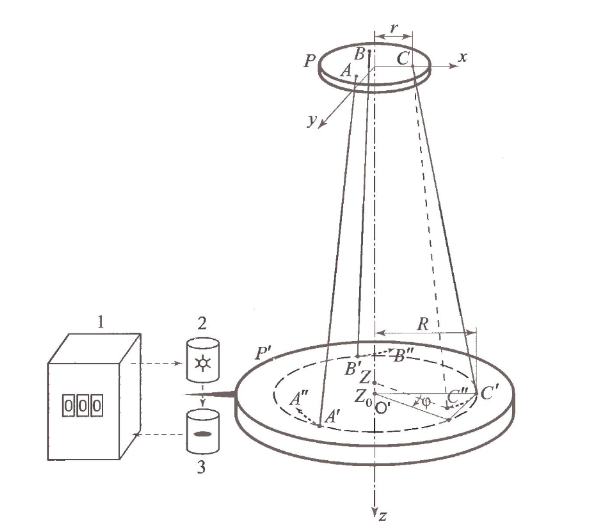
\includegraphics[width=0.95\linewidth]{pick1.PNG}
    \caption{Физический маятник}\label{risunok}
\end{wrapfigure}

Для наших целей удобно использовать устройство, показанное на Рис. \ref{risunok} и называемое трифилярным подвесом. Оно состоит из укрепленной на некоторой высоте неподвижной платформы $P$ и подвешенной к ней на трех симметрично расположеных нитях $AA'$, $BB'$ и $CC'$, вращающейся платформы $P'$. 

Чтобы не вызывать дополнительных раскачиваний, лучше поворачивать верхнюю платформу, укрепленную на неподвижной оси. После поворота верхняя платформа остается неподвижной в течение всего процесса колебний. После того, как нижняя платформа $P'$ оказывается повернутой на угол $\varphi$ относительно верхней платформы $P$, вощникает момент сил, стремящийся вернуть нижнюю платформу в положение равновесия, при котором относительный поворот платформ отсутствует. В результате платформа совершает крутильные колебания.


\par Инерционность при вращении тела относительно оси определяется моментом инерции тела относительно этой оси. Момент инерции твердого тела относительно неподвижной оси вращения вычисляется по формуле:

\begin{equation}
    I = \int r^2 dm
\end{equation}

Здесь $r$ -- расстояние элемента массы тела $dm$ от оси вращения. Интегрирование проводится по всей массе тела $m$.

Если пренебречь потерями энергии на трение о воздух и крепление нитей, то уравнение сохранения энергии при коебаниях можно записать следующим образом:

\begin{equation}\label{moment}
    \frac{I \dot{\varphi^2}}{2} + mg(z_0-z) = E
\end{equation}

Здесь $I$ -- момент инерции платформы вместе с исследуемым телом, $m$ -- масса платформы с телом, $\varphi$ -- угол поворота платформы от положения равновесия системы, $z_0$ -- координата по вертикали центра нижней платформы $O'$  при равновесии ($\varphi = 0$), $z$ -- координата той же точки при некотором угле поворота $\varphi$. Превый член в левой части уравнения -- кинетическач энергия вращения, второй член -- потенциальная энергия в поле тяжести, $E$ -- полная энергия системы (платформы с телом).

Воспользуемся системой координат $x, y, z$, связанной с верхней платформой, как показано на Рис. \ref{risunok}. Координаты верхнего конца одной из нитей подвеса точки $C$ в этой системе -- $(r, 0, 0)$. Нижний конец данной нити $C'$, находящийся на нижней платформе, при равновесии имеет координаты $(R, 0, z_0)$, а при повороте платформы на угол $\varphi$ эта точка переходит в $C''$ с координатами $(Rcos\varphi, Rsin\varphi, z)$. расстояние между точками $C$ и $C''$ равно длине нити, поэтому, после некоторых преобразований, получаем: 

\begin{center}
    \[ (R\cos\phi - r)^2 + R^2\sin^2\phi + z^2 = L^2 \]
    
    \[ z^2 = L^2 - R^2 - r^2 + 2Rr\cos\phi \approx z^2_{0} - 2Rr(1 - \cos\phi) \approx z^2_{0} - Rr\phi^2 \]
    
    \[ z = \sqrt{z^2_{0} - Rr\phi^2} \approx z_{0} - \frac{Rr\phi^2}{2z_{0}}\]
\end{center}

Подставляя $z$ в уравнение \eqref{moment}, получаем:

\begin{equation}
    \frac{1}{2}I\dot{\varphi^2} + mg \frac{Rr}{2z_0}\varphi^2 = E
\end{equation}

Дифференцируя по времени и сокращая на $\dot\varphi$, находим уравнение крутильных колебаний системы:

\begin{equation}
    I\ddot\varphi^2 + mg\frac{Rr}{2z_0}\varphi^2 = 0
\end{equation}
    
Производная по времени от $E$ равна нулю, так как потерями на трение, как уже было сказано выше, пренебрегаем.

Решение этого уравнения имеет вид:

\begin{equation}
    \varphi = \varphi_0 sin \left(\sqrt{\frac{mgRr}{Iz_0}}t + \theta\right)
\end{equation}

Здесь амплитуда $\varphi_0$ и фаза $\theta$ колебаний определяются начальными условиями. Период кртуильных полебаний нашей системы равен:

\begin{equation}
    T = 2\pi \sqrt{\frac{Iz_0}{mgRr}}
\end{equation}

Из формулы для периода получаем:

\begin{equation}\label{momin}
    I = \frac{mgRrT^2}{4 \pi^2z_0} = kmT^2
\end{equation}
\noindent где $k = \frac{gRr}{4\pi^2z_0}$ -- величина, постоянная для данной установки.
При возбуждении крутильных колебаний маятникообразных движений платформы не наблюдается -- устройство функционирует нормально.

При выводе формул мы предполагали, что потери энергии, связанные с трением, малы, то есть мало затухание колебаний. Это значит, что теоретические вычисления будут верны, если выполняется условие:
 \begin{equation}
    \tau \gg T
\end{equation}


\section{Результаты измерений и обработка данных}

1. Измерим параметры установки:

\begin{table}[!h]
\centering
\begin{tabular}{|c|c|c|}
\hline
$z_{0}$, cm & $R$, mm & $r$, mm \\ \hline
$213,6 \pm 0,5$  & $114,6\pm 0,5$  & $30,5\pm 0,5$                                                          \\ \hline
\end{tabular}
\end{table}

2. Вычислим константу установки по формуле:
\[\sigma_{k} = \sqrt{\sigma_{\text{сист}}^2 + \sigma_{\text{случ}}^2} = 0,005 \text{м}\]

\[k = \frac{gRr}{4\pi^2z_{0}} = 4,012*10^{-4} \pm 0,005 \text{м} \]
\newpage

3. Вычислим момент инерции пустой платформы:

\[I = \frac{mR^2}{2}= 7,33*10^{-3} \text{кг}*\text{м}^{2}\] 
\[\sigma_{I} = \sqrt{\sigma_{\text{сист}}^2 + \sigma_{\text{случ}}^2} = 0,7*10^{-3} \text{м}\]
\[I = (7,3\pm 0,7)*10^{-3} \text{кг}*\text{м}^{2}\]

4.Проведем серии экспериментов и на их основе рассчитаем моменты инерции: 

\begin{table}[!h]
\centering
\begin{tabular}{|c|c|c|c|c|}
\hline
$\text{Тело}$ & $\text{Измеренный период (10 колеб)}$ , c & $\text{Масса тела} , r$& $\text{Радиус тела}$, mm& $\text{Момент инерции}\text{ } \text{кг}*\text{м}^{2} $\\ \hline
$\text{пустой диск}$  &43,80  & $983,2$& 122,6&  $7,56*10^{-3}$  \\ \hline
$\text{кольцо}$  &41,66  & $777,5$& 76&  $5,40*10^{-3}$  \\ \hline
$\text{кольцо+диск}$  &39,03  & $1361,9$& 76&  $8,31*10^{-3}$  \\ \hline
$\text{диск}$  &39,18  & $584,4$& 170&  $3,60*10^{-3}$  \\ \hline
$\text{цилиндр}$  &37,23  & $1200,0$& 7,45&  $6,66*10^{-3}$  \\ \hline
$\text{разрез. диск}$  &30,72  & $1442,2$& 38,8&  $5,45*10^{-3}$  \\ \hline
\end{tabular}
\end{table}

Т.к практическая погрешность складывается только из массы, периода и k , то для всех она будет одинакова и равна :
\[\sigma_{\text{пр}} =\sqrt{\sigma_{\text{сист}}^2 + \sigma_{\text{случ}}^2} = 0,021  \]
Рассчитаем теоретические моменты инерции для кольца, диска и цилиндра:
\[I_{k} = mr^{2} = 4,67  \text{кг}*\text{м}^{2}\]
\[I_{d} = \frac{mR^2}{2} = 2,8  \text{кг}*\text{м}^{2}\]
\[I_{c} = \frac{mR^2}{2} = 5,9  \text{кг}*\text{м}^{2}\]

Рассчитаем моменты инерции для половинок диска:

\begin{table}[!h]
    \centering
    \begin{tabular}{|c|c|c|c|}
    \hline
$\text{Раздвиг}, mm$ & $\text{Измеренный период (10 колеб)}$ , c & $\text{Масса тела} , r$& $\text{Момент инерции}\text{ } \text{кг}*\text{м}^{2} $\\ \hline
$\text{0,5}$  &30,78  & $1442,2$&   $5,48*10^{-3}$  \\ \hline
$\text{1}$  &30,88  & &   $5,52*10^{-3}$  \\ \hline
$\text{1,5}$  &31,21  & &   $5,63*10^{-3}$  \\ \hline
$\text{2}$  &31,63  & &   $5,77*10^{-3}$  \\ \hline
$\text{2,5}$  &32,14  & &   $5,96*10^{-3}$  \\ \hline
$\text{3}$  &32,71  & &   $6,18*10^{-3}$  \\ \hline
\end{tabular}
\end{table}

По этим данным построим график $I(h^{2})$:

Через апроксимацию находим накл коэф прямой, оттуда при h = 0, $I=5,45*10^{-3}  \text{кг}*\text{м}^{2}$ , коэффициент наклона равен 0.812 \par
Из графика масса диска равна 1390 г что составляет $96\%$ от истинного значения
\newpage

\begin{figure}[h!]
\centering
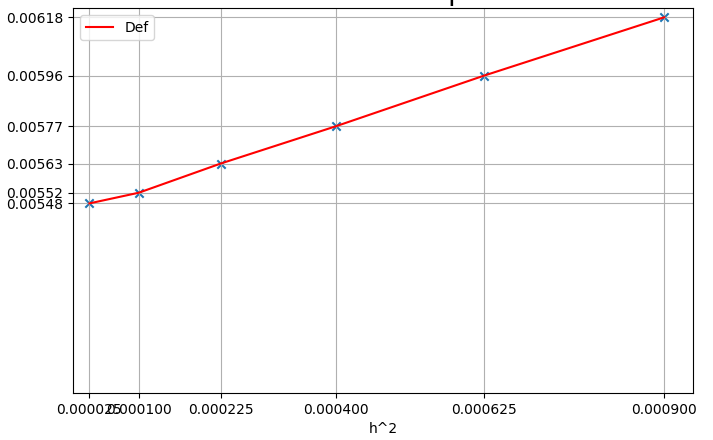
\includegraphics[width=1\textwidth]{pick3.PNG}
\caption{График I от $h^{2}$}
\end{figure}




\end{document}